\section{A Chemistry case study}\label{sec:chemcase}
To conclude we apply many of the tools described above to a simple case study. We select a MCM subset containing methane as the only primary emitted species, and run it throught the Dynamically simple model of atmospheric chemical complexity (DSMACC) [ref] using the initial conditions of XYZ. We run this forwards to steady state and extract the flux between species on noon. The edge weight is the net flux (product of the species concentration * the rate of reaction for all reactions), normalised to a value between 1 and zero. 

This allows a simplified view of the different properties which affect the visualisation of the graph produced. 

\subsection{Syntatic representation} 
Since we shall be using simulation data, we require a layout which deals with both direction and edge weights. In the spirit of zero and Protagoras\footnote{Famous for the phrase `man is the measure of all things' suggesting that we are constrained by our experiences}, we opt of the spring-like description presented by the Force Atlas 2 algorithm. This feature hi-lights fast reactions by bringing nodes together. Such a property has been observed to help users select the shortest path within a network, \cite{eyetrack}. Here users picked the shortest path an average of 68\% for force directed graphs, compared to 40\% for hierarchical and 2\% for orthogonal layouts. Such properties can help us locate any trends in fast reactions which may control the chemistry within a system. 


\subsection{Semantic representation}
Since the graph presented contains only a handful of species, our screen real-estate allows the listing of names for each node. Node sizes are scaled to represent the concentration of each species at that time point, and edges are coloured to represent the strength of each relationship between them. 


\begin{figure}[H]
     \centering
    \begin{subfigure}[b]{.4\textwidth}
         \centering
     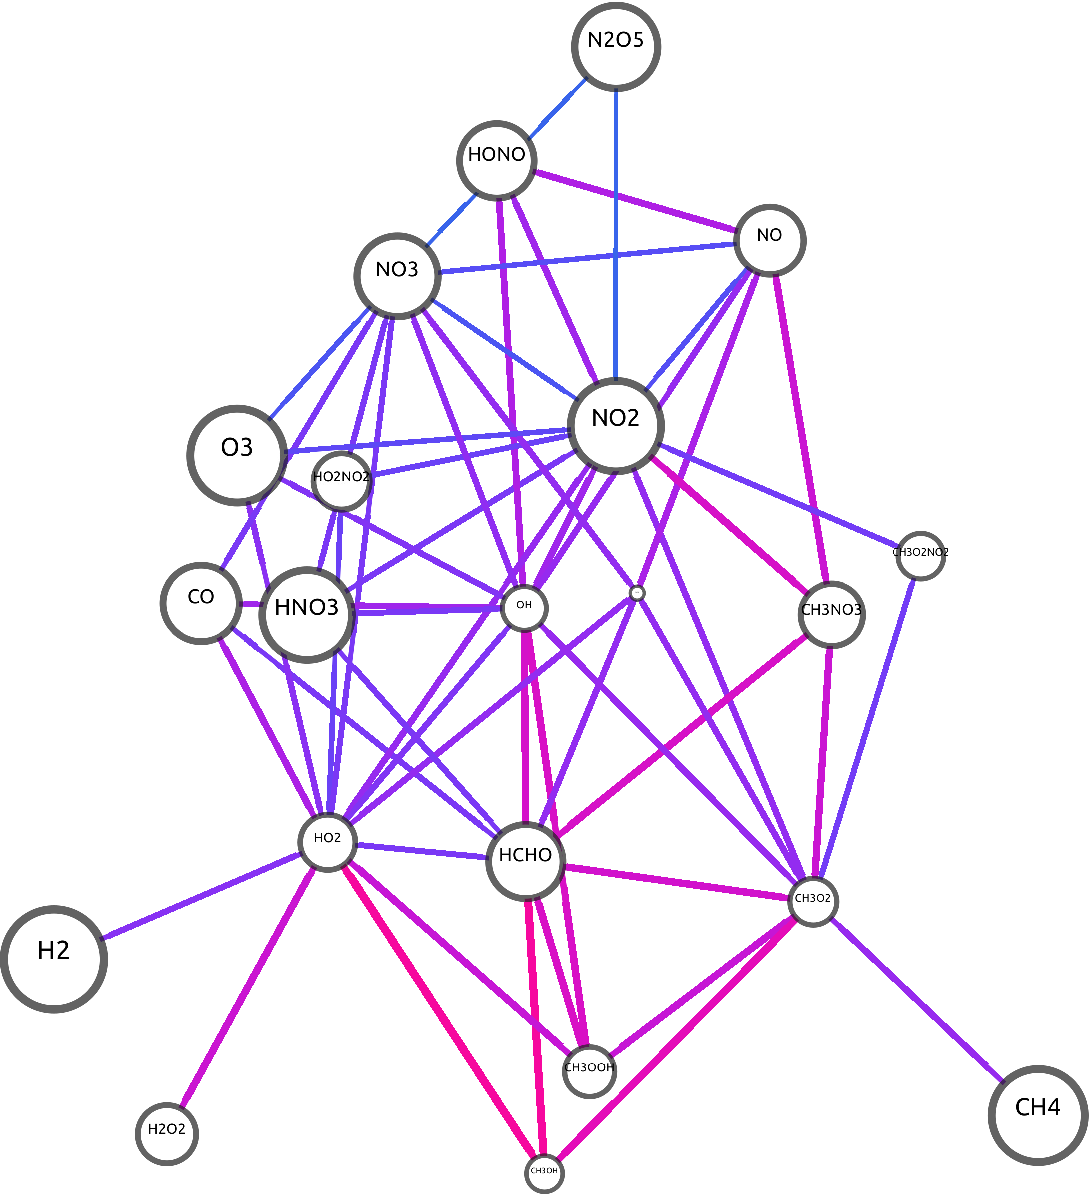
\includegraphics[width=\textwidth]{figures_c1/tap3/ch4_stretcheddefault-eps-converted-to.pdf}
     \caption{Connected unweighted}
     \end{subfigure}
     \begin{subfigure}[b]{.4\textwidth}
         \centering
     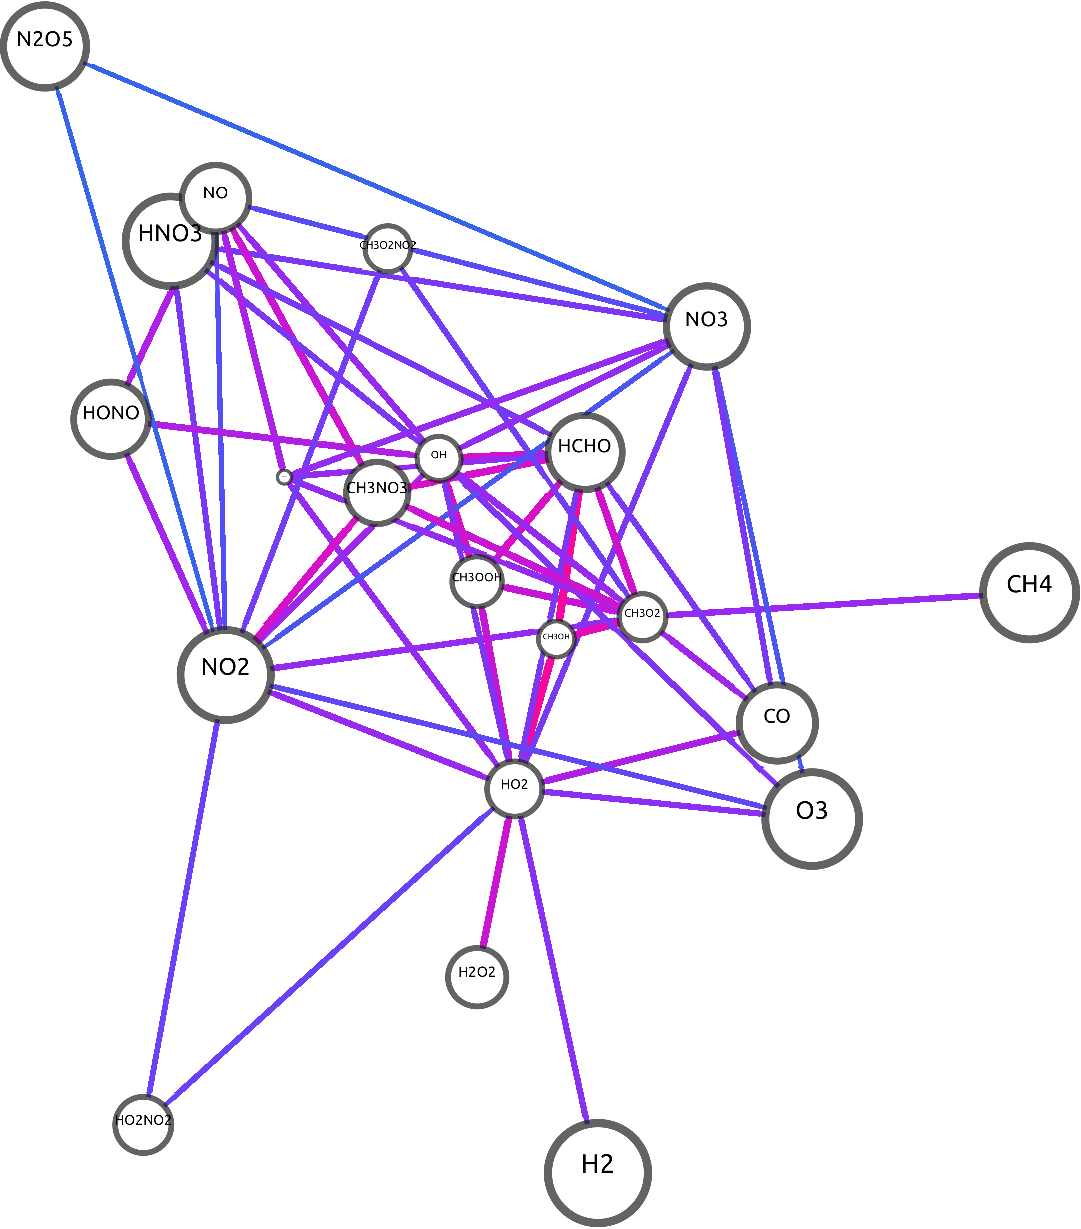
\includegraphics[width=\textwidth]{figures_c1/tap3/ch4_weighted_s1-eps-converted-to.pdf}
     \caption{Connected $\hat{\Gamma} = flux$}
     \end{subfigure}
        \caption{Basic steps within in the the graph production process}
      \label{fig:resmeth}
\end{figure}

\subsection{Local vs Global minimum }
Since computers are deterministic, so are the calculations they perform\footnote{Within a certain precision...}. In starting nodes from the same physical location and exerting the same force upon them, a force directed simulation will result in the nodes settling in the same locations. Since we use this `final' resting as the basis of our visual analysis, it is important to find out if it represents the global minimum of the graph, or is merely a combination of the layout parameters and random seed. 

To do this we take a selection of 360 randomly initiated simulations, applying a monte carlo approach to simulation parameters and initial node placement. The force directed algorithm is then allowed to run with progressively decreasing energy until it reaches a stable equilibrium. Once this has been done we 

To ensure a global minimum has been met, a monte carlo approach with initial conditions is employed. Since a graph may hold both symmetrical and rotational symmetry, it is necessary to constrain the number of degrees of freedom it contains. The simplest way to do this would be to fix several nodes, and allow the force graph to evolve around this. Here we select the NO$_x$ species,$\{NO, NO_2,NO_3\}$, since their links form a triangle, and in doing so we can eliminate the rotational component of the algorithm. 

From here we allow the force directed algorithm to run until the nodes have settled, and record their positions. Once this has been done, all non-fixed nodes are given a random position and this whole process is repeated. 


\subsubsection{Approximation of degrees of freedom} 
Nodes with no connections can exist anywhere. Nodes which only have one connection, can only exist within a circle from the node they are bound to. If a node is connected  to two other nodes, it must therefore exist somewhere between them. This means that in general the more links a node has (its degree), the more constrained its location within the graph layout. 


\begin{figure}[H]
    \centering
    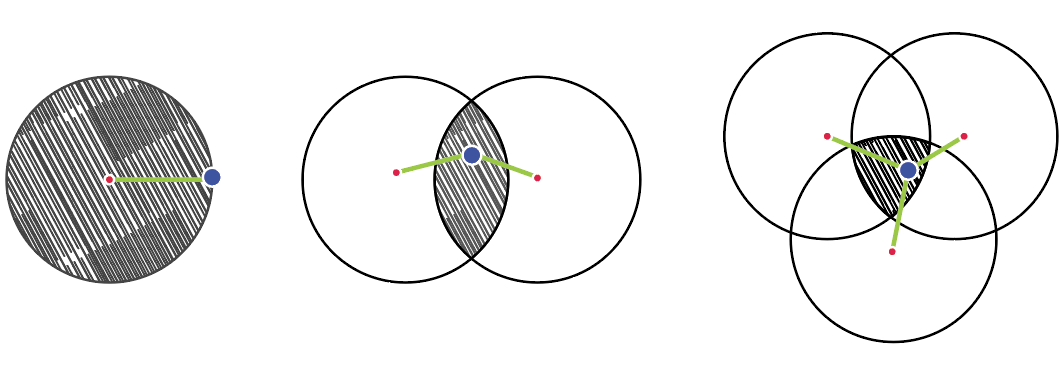
\includegraphics[width=.8\textwidth]{figures_c1/circles.png}
    \caption{A demonstration on how the area / degrees of freedom (grey hashed area) of a node (blue) are limited by the number of neighbouring nodes it is anchored to (red) }
    \label{fig:circle}
\end{figure}

To test this we compare node degree with the dispersion between nodes in the above setup of the methane model. However since graphs are muli-link systems, the number of local minima for a specific node is not limited to direct links to its neighbours, their neighbours and so forth. To take this into account we device an \textit{approximate} metric - outlined below. 

\paragraph*{ A metric of establishing how mobile a node is within the force graph layout}
As with all mathematical approximations we begin using a set of axioms. For this example we assume that: 
\begin{itemize}
    \item[1.] We have a set of fixed species, which we use to constrain the rotational symmetry of the graph with. In this case they are the NO$_x$ species.
    \item[2.] A nodes `freedom' is mostly determined through the shortest path to all fixed species. 
    \item[3.] We calculate the freedom by propagating the fraction of this constraint based on the number of links for each node, and propagating this forwards through the system
    \item[4.] This metric is used as an effective indicator and not a complete calculation (where all possible paths should be used)
\end{itemize}

\paragraph*{A worked example}
To demonstrate this example we take an example shortest path (A-B-C-D) where A is fixed. Here B has 2 links, C has 3 and D has 4. The calculation of the freedom of D therefore equates to:
\begin{center}
\begin{multline} \\
    A_{dof}  = 1\ (A\  fixed\  node)\\
    B_{dof}  = A_{dof} /  2 = 1/2\\
    C_{dof}  = B_{dof} /  3 = 1/6\\
    D_{dof}  = C_{dof} /  4 = 1/24\\
\end{multline}
\end{center}
 Finally inverse the values ($1-D_{dof}$) - such that the greater the output, the more freedom a node has in its final destination. 
 
 \paragraph*{Plotting correlation}
 Using a setup of the $NO_{1-3}$ species (the red nodes: \autoref{fig:frmd_setup}) constrained in a triangle we run 1200 randomly initiated force directed graphs for the methane network and map the local minima obtained by each node at the end of each one.
 
  We then use this to calculate the deviation between each of these resting positions, their degree of freedom metric output and the node degree for each one. In looking only at the nodes connected to at-least one of the three fixed species, \autoref{fig:frmd_nox}, we see a pattern similar to that of \autoref{fig:circle}. Here the species \ce{CO,CH3O2NO2,HO2NO2} and \ce{CH3O2} all have a single link to a fixed species, and can disperse themselves evenly around these. Species with links to two fixed species, \ce{N2O5,HONO,O3,CH30} and \ce{CH3NO3}, are bulled between the two $NO_x$ species that they react with. Finally we have the hydroxide radical which reacts with all of the fixed species and is located at the centre of the triangle\footnote{As a note to clarify: although \ce{CH3O2} reacts with all three fixed groups, the construction methodology for this specific graph only take reactant-product pairs into account. As all of these are reactant-reactant reactions, they are not included within the graph.}.
  

\begin{figure}[H]
     \centering
      \begin{subfigure}[b]{.38\textwidth}
         \centering
     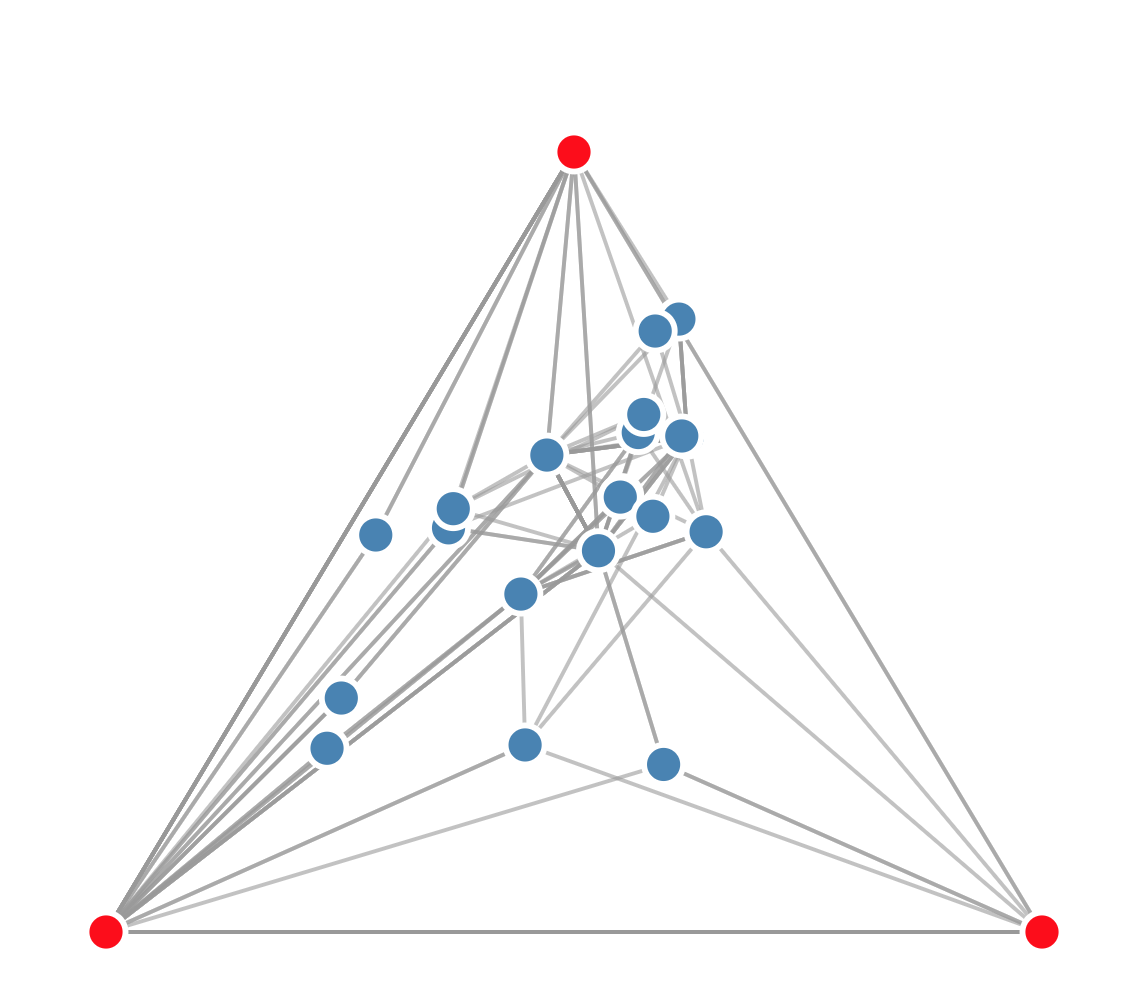
\includegraphics[width=\textwidth]{figures_c1/frmd.png}\vspace*{+8mm} 
     \caption{The complete graph}
     \label{fig:frmd_setup}
     \end{subfigure}
    \begin{subfigure}[b]{.45\textwidth}
         \centering
     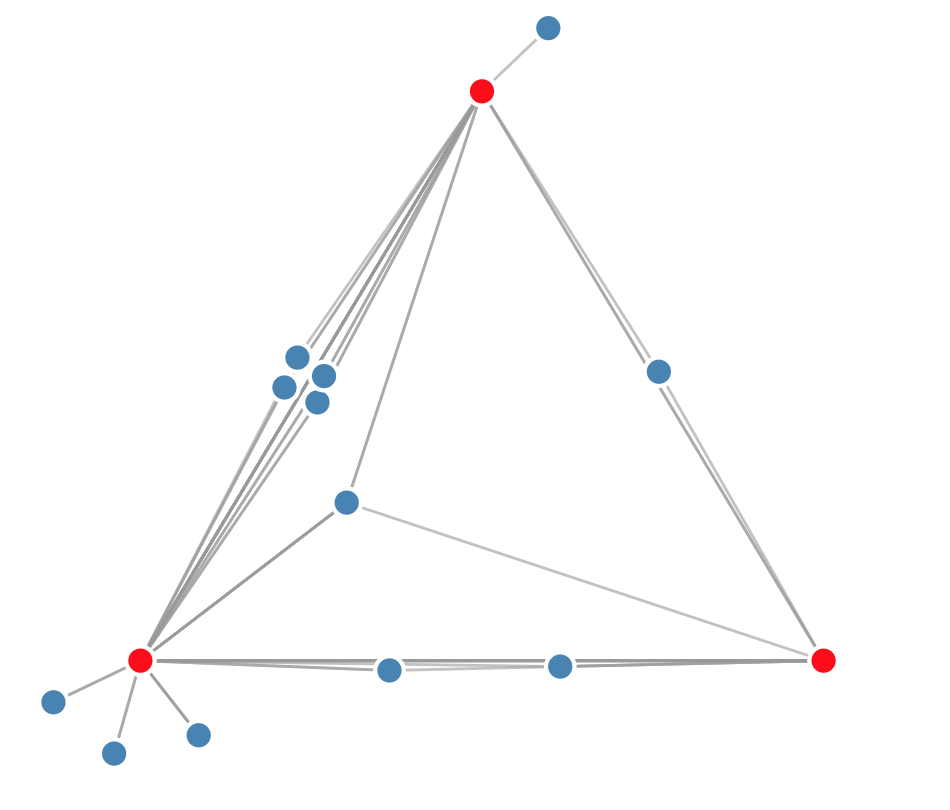
\includegraphics[width=\textwidth]{figures_c1/frmd2.png}
     \caption{Fixed node adjacent}
     \label{fig:frmd_nox}
     \end{subfigure}
    %  \begin{subfigure}[b]{.32\textwidth}
    %      \centering
    %  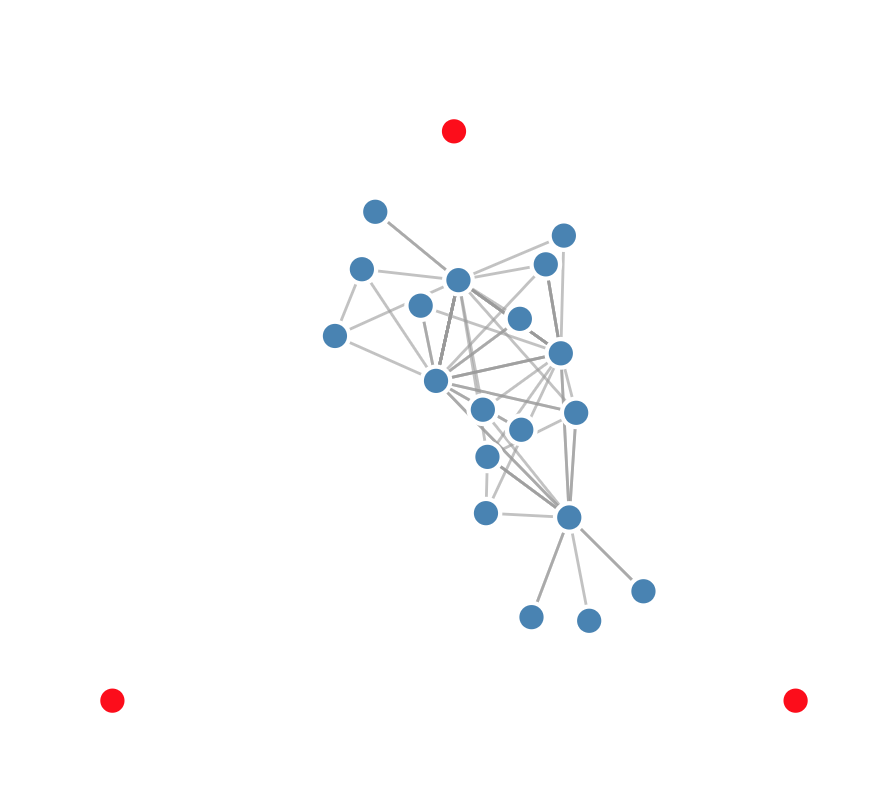
\includegraphics[width=\textwidth]{figures_c1/frmd3.png}
    %  \caption{Fixed node independant}
    %  \label{fig:frmd_nonox}
    %  \end{subfigure}
        \caption{Showing the experimental force graph setup, with NO \ce{NO2} and \ce{NO3}  (red) fixed in position (\ref{fig:frmd_setup}). This     }
      \label{fig:frmdstart}
\end{figure}
 
 
 To plot the correlation we use a Force Directed Representation of Multivariate Data (FRMD), written to show relationships between variables for data \cite{frmd}. This takes multivariate data and plots it in a inverse, fully connected graph\footnote{This is similar to the t-SNE dimensionality reduction technique [REF SECT]}. \autoref{fig:frmd_full} shows the a three dimensional comparison between a species deviation in resting position, degree and metric value.  Here nodes are connected to each category with a series of fixed `rods` or links. The length of each rod is adjusted such that it reflects the normalised value of its influence due to its origin category. This works by effectively `pushing` the node towards its category name. This allows us to partition the data into groups with similar properties, or extremes - for example \ce{CH3O2,HO2} and OH all have high degree values (>10 links) and low deviation in their local minimia locations. \ce{H2, CH3OH, CH3OOH} on the other hand have a wide range of possible local minima (deviation), which may be attributed to their low degree values. Formaldehyde on the other hand has both a high location deviation, as well as degree in general. These results suggest that for the higher metric values (small node size and near the bottom due to the 1-metric data set) the results are split between highly constrained species (due to a large number of links and a small deviation) and those which have many local minimia, and few links. 
 
 
 
 \begin{figure}[H]
     \centering
     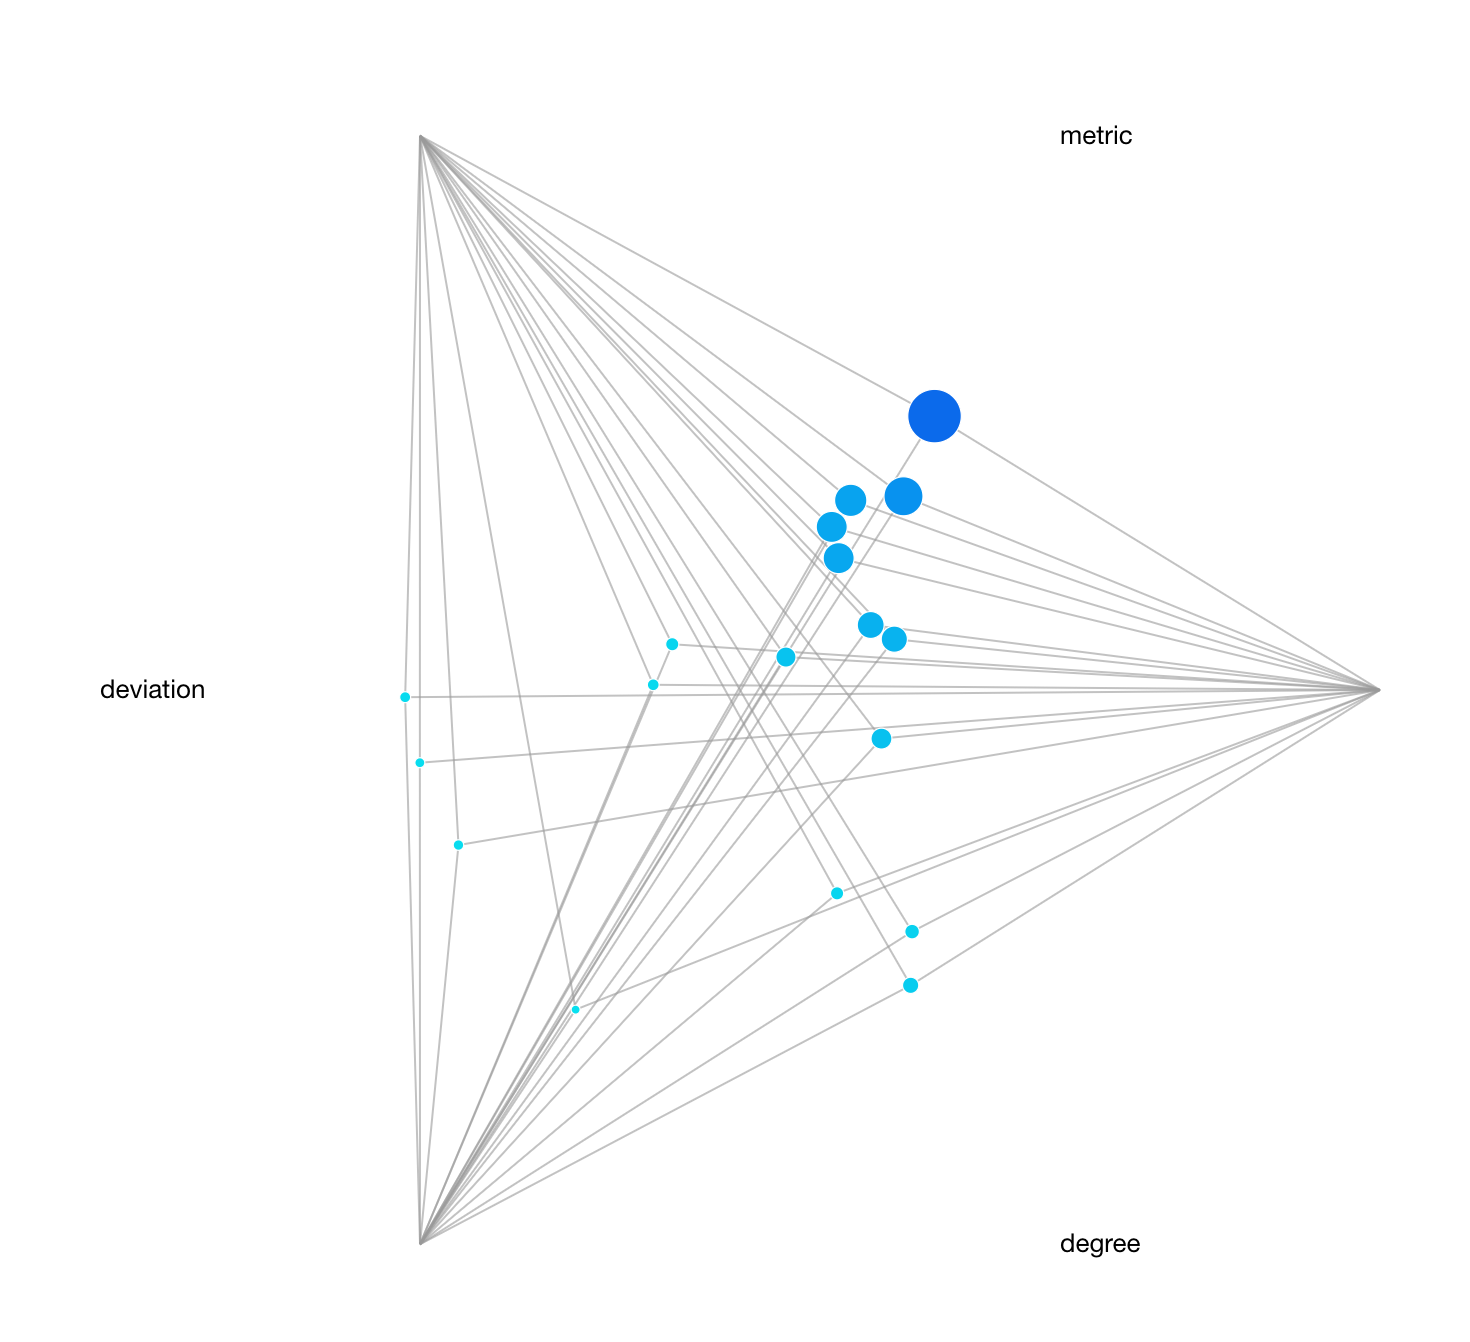
\includegraphics[width=.8\textwidth]{figures_c1/fullold.png}\vspace*{+0mm} 
     \caption{A plot showing the relationships between all three categories, and the links between them. Here we may identify groups of similar relationships, with the nodes close to a title having a high value in that feature, and ones near the middle containing a high value for all variables. \textbf{Values for the metric are 1-metric for this example.} }
     \label{fig:frmd_full}
     \end{figure}
     
     We can also reduce the number of dimensions of the FRMD visualisation from 3 to two. In taking only two features and encoding the third through either size or colour we can sometimes present a clearer correlation between items. Within these visualisations we have imbalanced nodes on the horizontal, with higher values pushing the node towards its respective label. In cases where the relationship is approximately equal with both features the nodes exist on the vertical plane between each feature. Here low ranked equality lies close to the center line. Higher correlated matches are result in rods longer than the horizontal distance between both features. This causes a vertical displacement separating the nodes from the horizontal. 
     
     \autoref{fig:frmd_devdeg} shows the relationship between the location deviation and a nodes degree. Here, as with the 3 dimensional plot, we have a group of species which have a low degree coupled with a high location deviation, and a set of highly constrained species with >10 links. Similarly \ce{HCHO}, having a high number in both, is pushed away from the horizontal. As the metric value is encoded in the colour, we see that this has a stronger correlation with degree than deviation, which is expected since this plays a central role in the calculation of the freedom metric. 
     
    \begin{figure}[H]
         \centering
     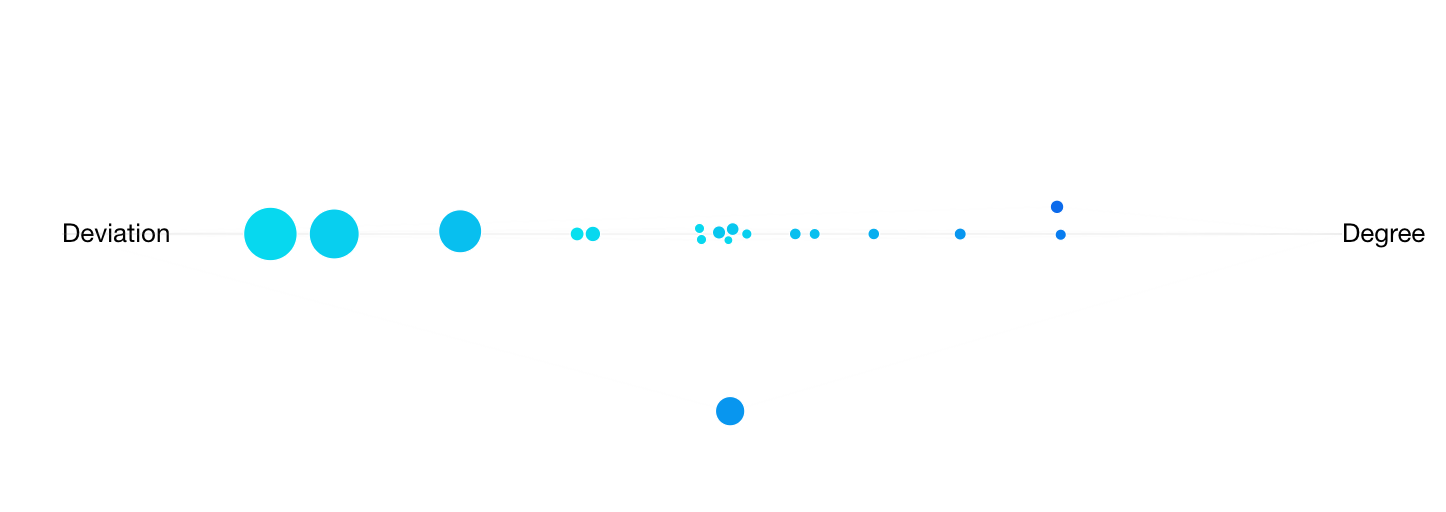
\includegraphics[width=\textwidth]{figures_c1/devdeg.png}
     \caption{Comparing deviations in node location with the number of links that species has within the reaction graph (degree) using a 2D version of the FRMD software. A node's importance with respect to the metric is embedded within the nodes colour and size.}
     \label{fig:frmd_devdeg}
     \end{figure}

    

Having seen how node degree fares against the actual deviation of each node, it is time to compare this against our metric. In \autoref{fig:frmd_devmet} we see a much narrower band of nodes along the horizontal. This suggests a greater correlation between the two values - the ranking within each category are of a similar magnitude. 


     \begin{figure}[H]
         \centering
     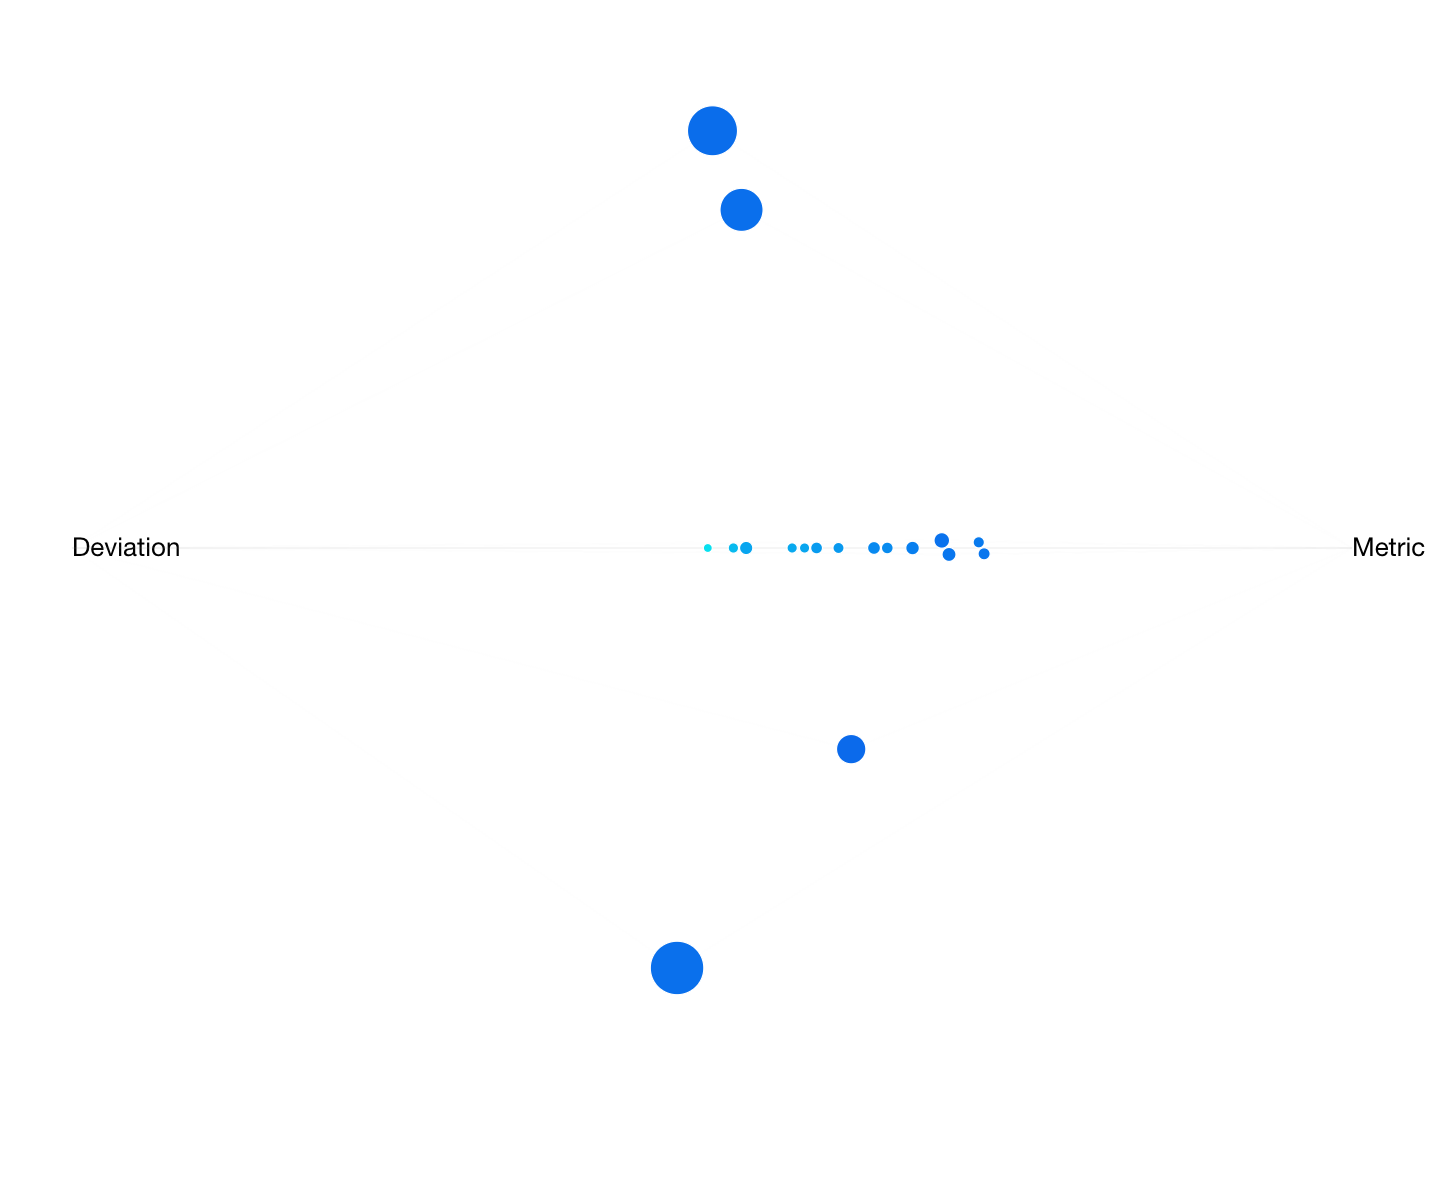
\includegraphics[width=\textwidth]{figures_c1/frmd_devmet.png}
     \caption{Exploring how node deviation varies with the freedom metric above. Node colour and size represent the degree of each node, and are represented using the FRMD model. }
     \label{fig:frmd_devmet}
     \end{figure}
 
 
 
 
 
 \newpage

%trim={<left> <lower> <right> <upper>}


\subsection{A model of Beijing}
Using a spun up model initiated from the campaign results XX Beijing (Where did I get these?) we compare the distribution of links within a model. In f[FIG XX] we see the graph shape change due to the presence of photons. 


To perform a sensitivity study on the initial positions of nodes within the force atlas algorithm, a graph consisting of links and weightings is constructed using a box model simulation of the Beijing summer environment at mid-day and feed it the gephi software, \cite{gephi} - an open source software designed for the exploration of networks. We then scrip the java code to perform the functions in \autoref{fig:flowrepeat}. As part of this, nodes are initiated with a random position, the force atlas 2 layout is then run and then the graph is rotated and translated such that it is centred around carbon monoxide and has a 45 degree angle between this and formaldehyde. This step constrains the general orientation of the graph, allowing us to analyse the generated graphs for global and local minima. The final step is to save a copy of the generated graph layout and repeat to generate a data set, a subset of which is shown in  \autoref{fig:all}

    \begin{figure}[H]
         \centering
     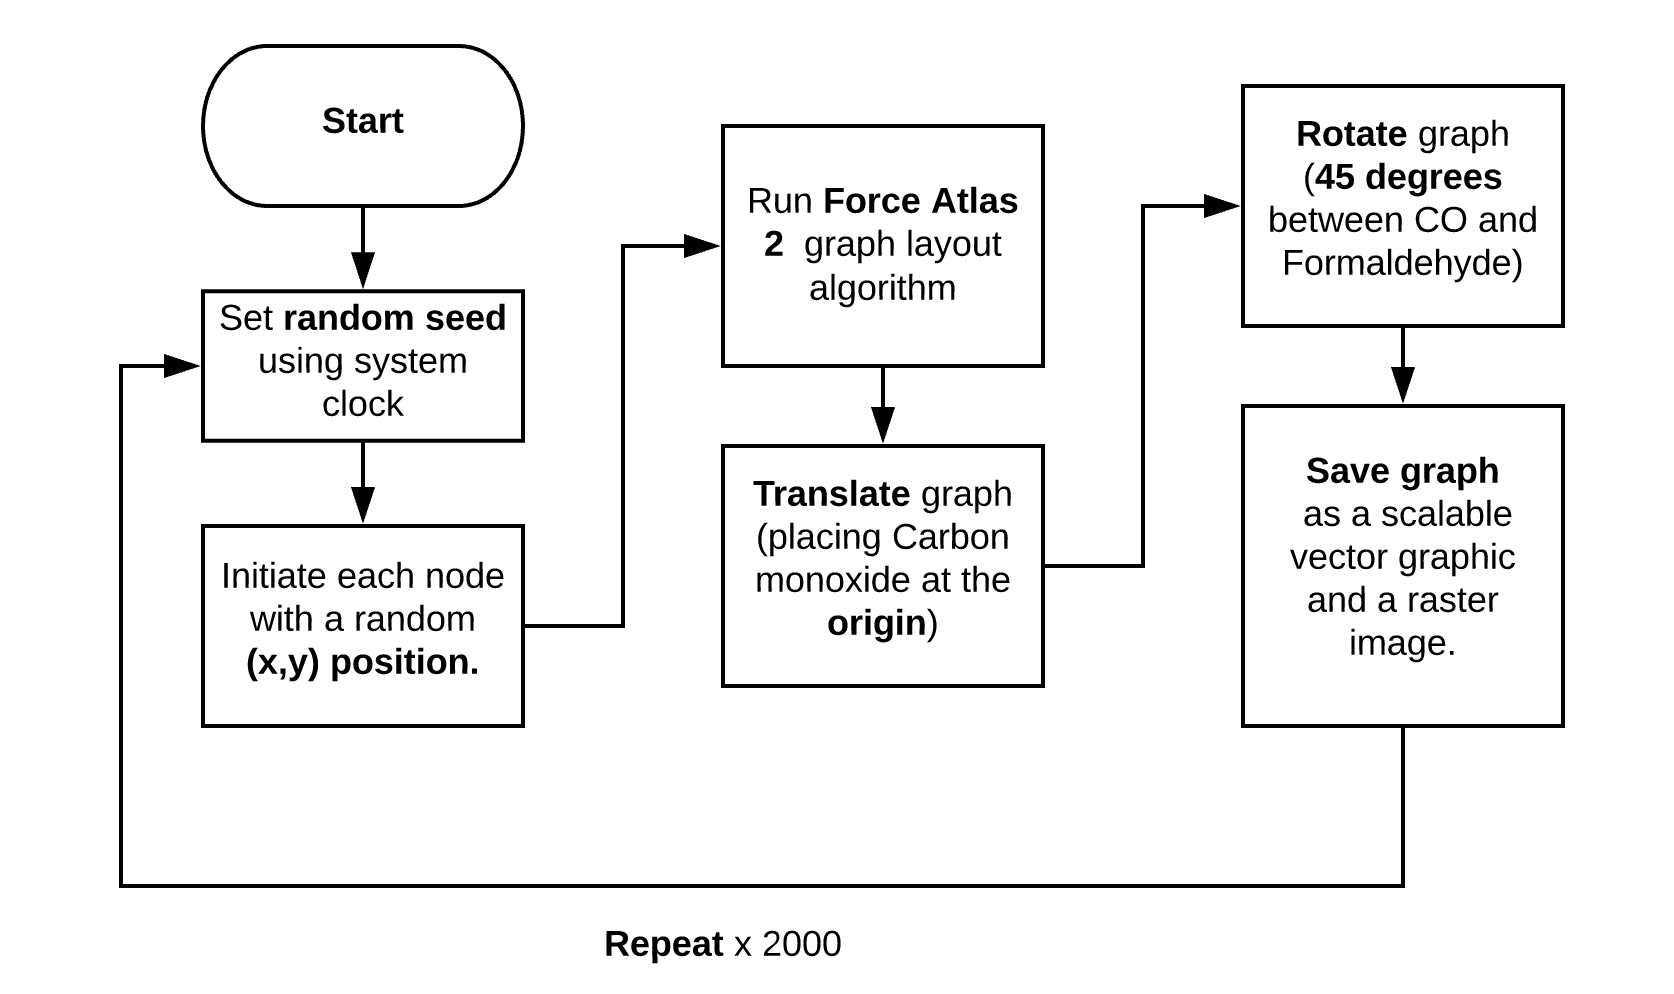
\includegraphics[width=\textwidth]{figures_c1/flowrepeat.png}
     \caption{ A flow chart of the process performed by the custom gephi script used to generate the data set}
     \label{fig:flowrepeat}
     \end{figure}
 
    \begin{figure}[H]
         \centering
     \includegraphics[width=\textwidth]{figures_c1/beijingtest/10_900.png}
     \caption{A sample of the 900 graphs generated using the force atlas 2 algorithm for the simulation output representative of the summer beijing chemistry at noon.  }
     \label{fig:all}
     \end{figure}
 

\subsubsection{Trends in the Chemistry}
Due to the construction protocols of the master chemical mechanism, \autoref{fig:protocol}, primary emitted compounds are oxidised to produce a cascade of species, ultimately ending at carbon dioxide\footnote{The MCM conserves the number of carbons, allowing \ce{CO2} to be introduced.} and water. As this process is central to the construction of the mechanism, it follows that they may be used to explain any features uncovered using the network layout. 

\paragraph{Network shape}\label{sec:netshape}
Using \autoref{fig:all} the pattern recognition capabilities of the human mind identify a certain shape associated with many of the networks. Upon closer inspection it may be hypothesized that the chemistry is split into three main branches. \autoref{fig:colour} categorises all the primary emitted species, and then uses voronoi tessellation\footnote{see chapter xxx for an example of this} to colour neighbouring nodes and their links by the classification of the closest primary emitted species. Using this it is possible to separate the MCM network into an aromatic branch, a terpene branch, an alkane and straight chain alkene branches. Such branches not only help us identify changes of chemistry due to biogenic or anthropogenic sources, but also emphasise the path taken to carbon dioxide and water. Since the MCM does not contain \ce{CO2} we see all the different groups converge on Carbon Monoxide (white, centre). Using this format, we may now compare the orientation of the many automatically generated layouts.  
 
    \begin{figure}[H]
         \centering
    %  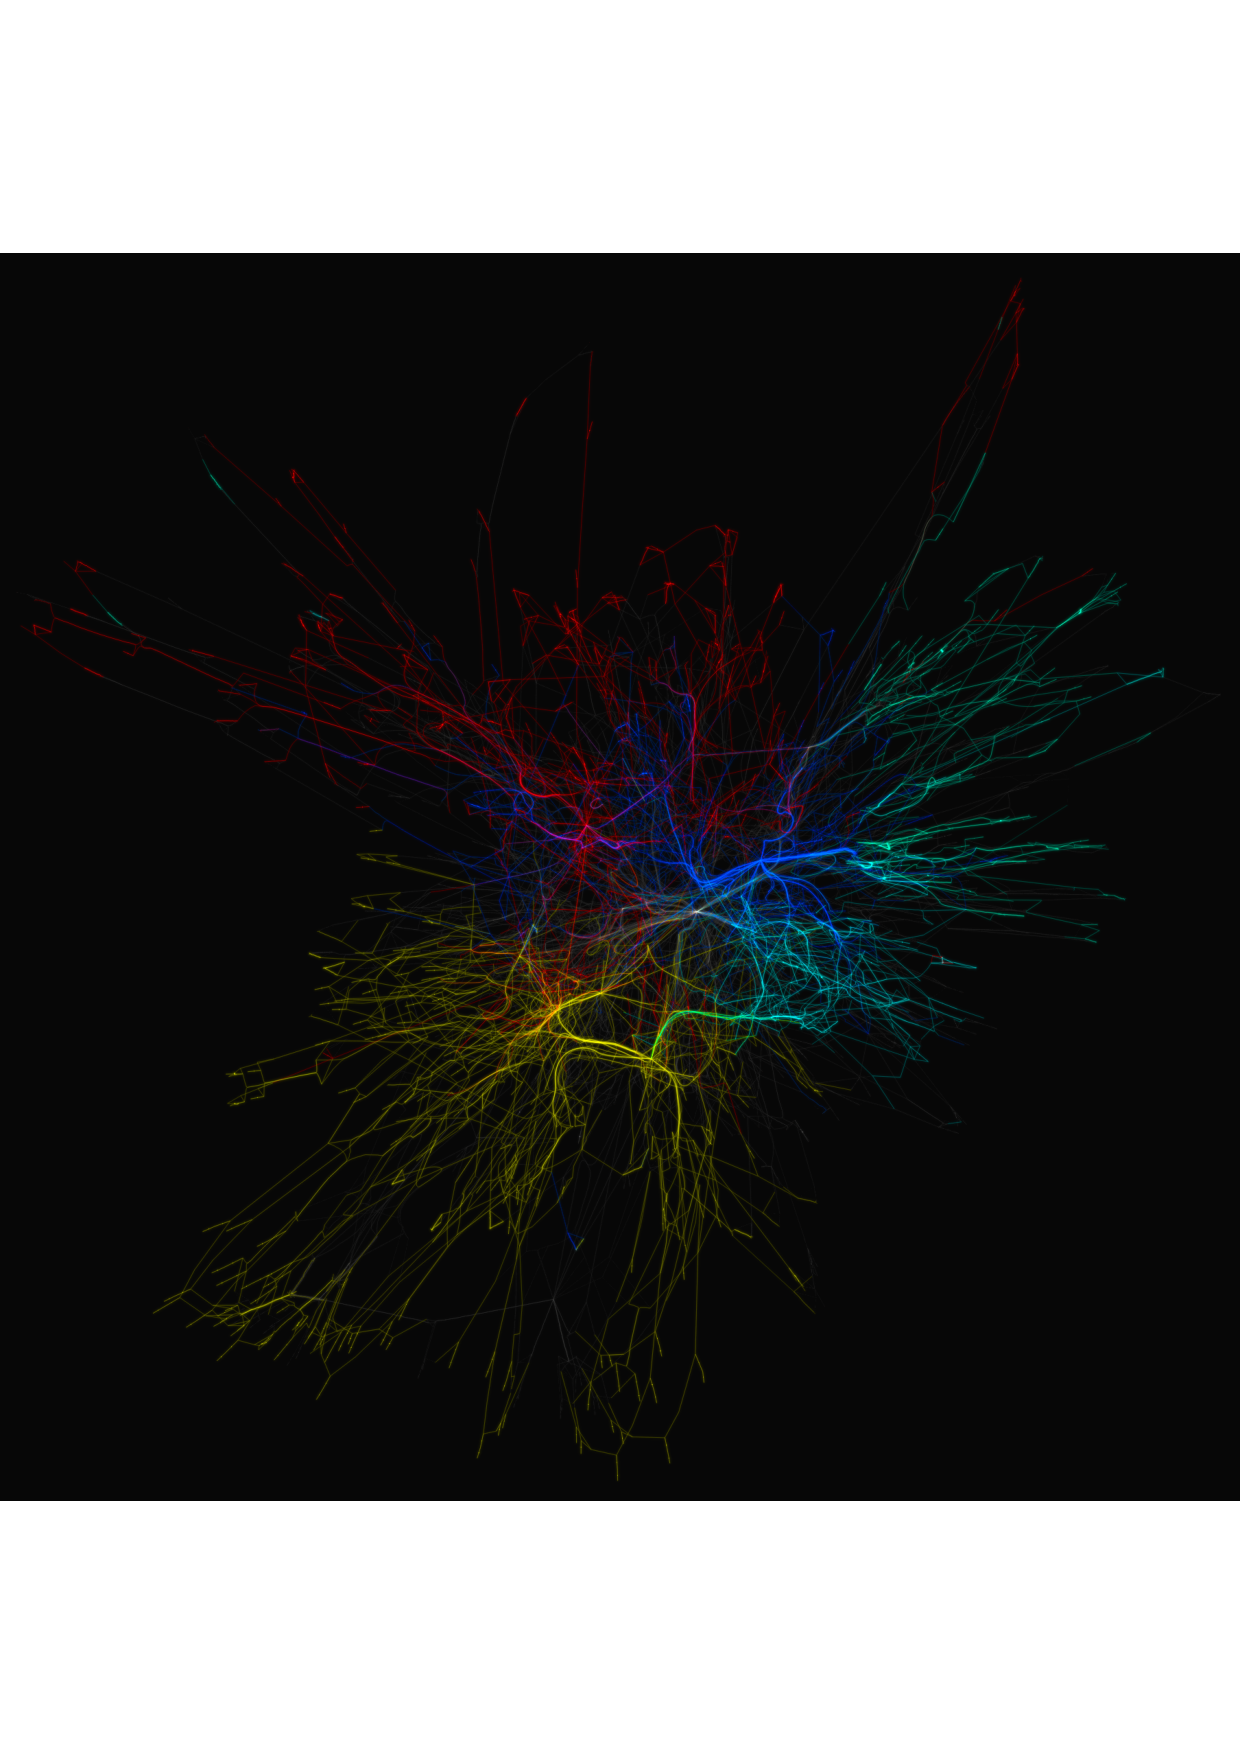
\includegraphics[width=\textwidth,trim={0 4cm 0 4cm}]{figures_c1/beijingtest/graphgroups.pdf}
    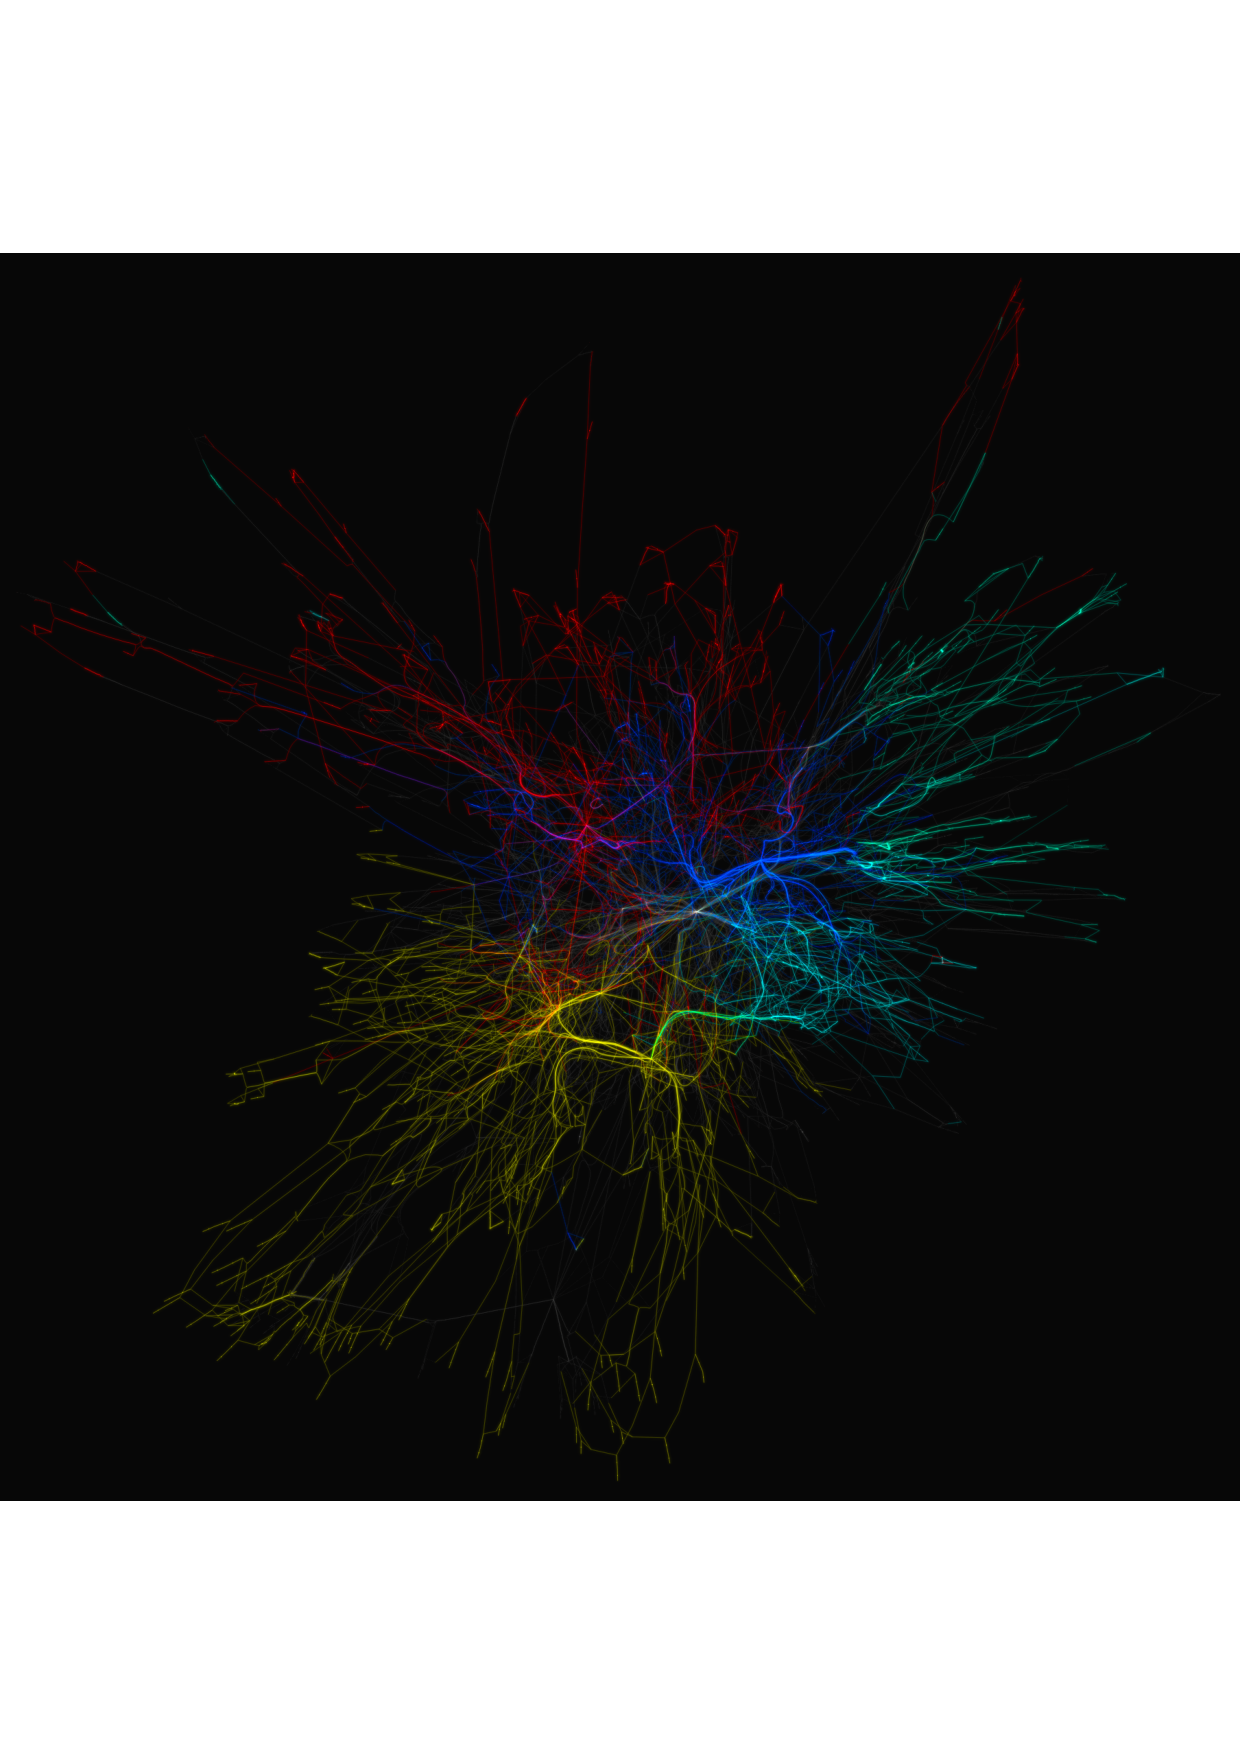
\includegraphics[width=\textwidth,trim={0 4cm 0 4cm},angle=-90]{figures_c1/beijingtest/graphgroups.pdf}
     \caption{Hi-lighting the groups of species, and their products within the MCM network graph. These are {\color{DarkGoldenrod} Aromatics (gold)} , {\color{DarkTurquoise} terpenes (turquoise) } and {\color{OrangeRed} Alkane}/{\color{RoyalBlue} Alkene  } carbon chains (red/blue)}
     \label{fig:colour}
     \end{figure}

\paragraph{Pattern Matching using t-SNE}
t-Distributed Stochastic Neighbor Embedding (t-SNE) is a dimensionality reduction technique used in automatic categorisation of images or photographs \cite{truthandbeauty,sketchy}. This is the same process as referenced in EARLIERREF and described in detail within Chapter... 

To compare the generated networks, we flatten the pixel matrix for each centered image in the dataset, and assign the output list to each filename. The resultant dataframe is then fed into the t-SNE algorithm in the Scikit Learn package, \cite{scikit-learn}. This reduces the logical list of pixels for each image into a two dimensional representation of their similarity. We plot each file, for its $(x,y)$ coordinate, and isolate clusters of similarity using density contours in 

    \begin{figure}[H]
         \centering
    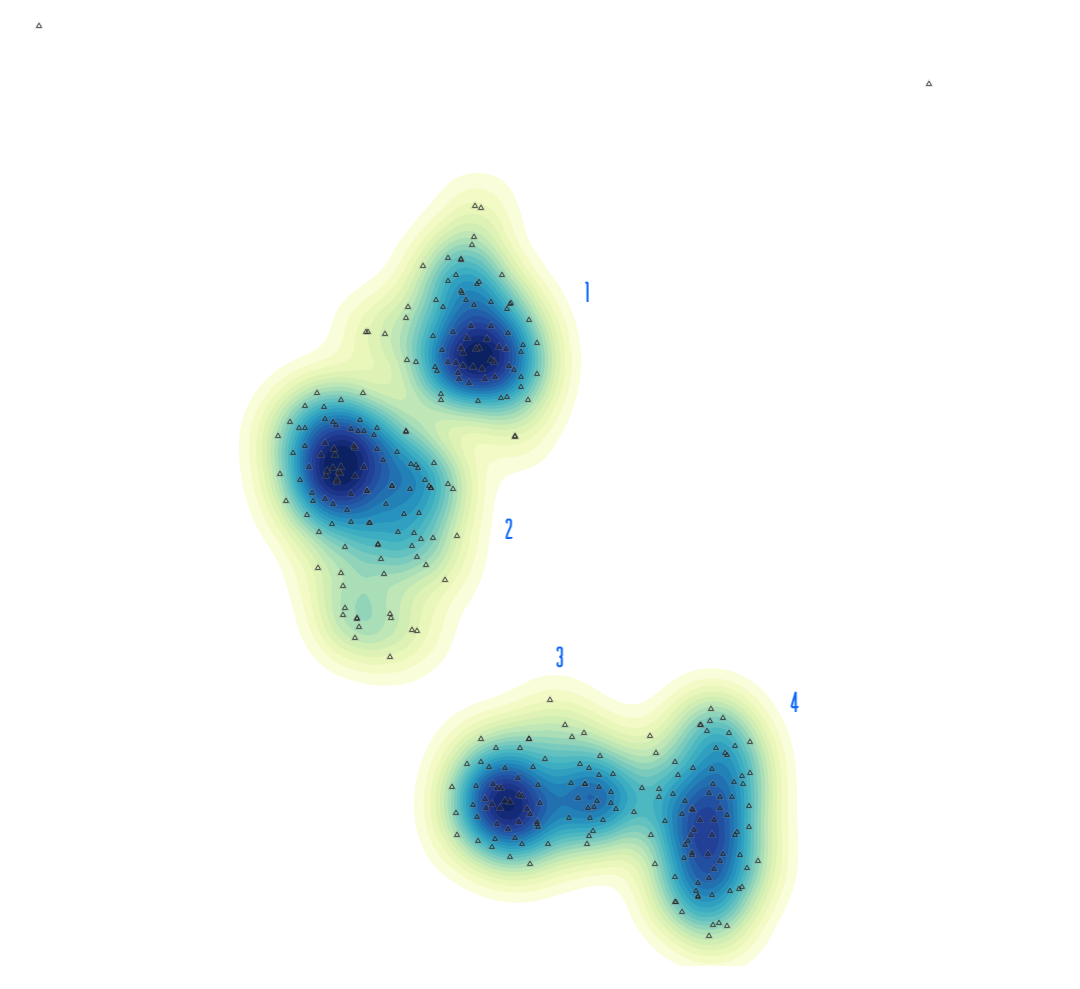
\includegraphics[width=.6\textwidth]{figures_c1/beijingtest/density.png}
     \caption{\textbf{A normalised scatter plot of 2D space produced by the t-SNE algorithm.} Each triangle represents a different file, and the colours/density contours show the regions in which we find similar images/graphs. }
     \label{fig:densty}
     \end{figure}

Using interactivity and/or vector cluster detection techniques it is possible examine which files contribute to an area of high density. \autoref{fig:densitypic} shows a sample of four graphs from each corresponding cluster. Although individual node locations may vary, patterns on the macro scale start to emerge, with similar groups exhibiting symmetrical symmetry, e.g. groups 1/2 and 3/4. This suggests a constraint in the overall degree of freedom can be attributed solely to the network structure, and consequently the chemistry which forms this. The non-random nature of the produced graph layouts mean that it would be possible to juxtapose a variety or mechanisms using the force atlas 2 layout.

\begin{figure}[H]
     \centering
     \begin{subfigure}[b]{.2\textwidth}
         \centering
     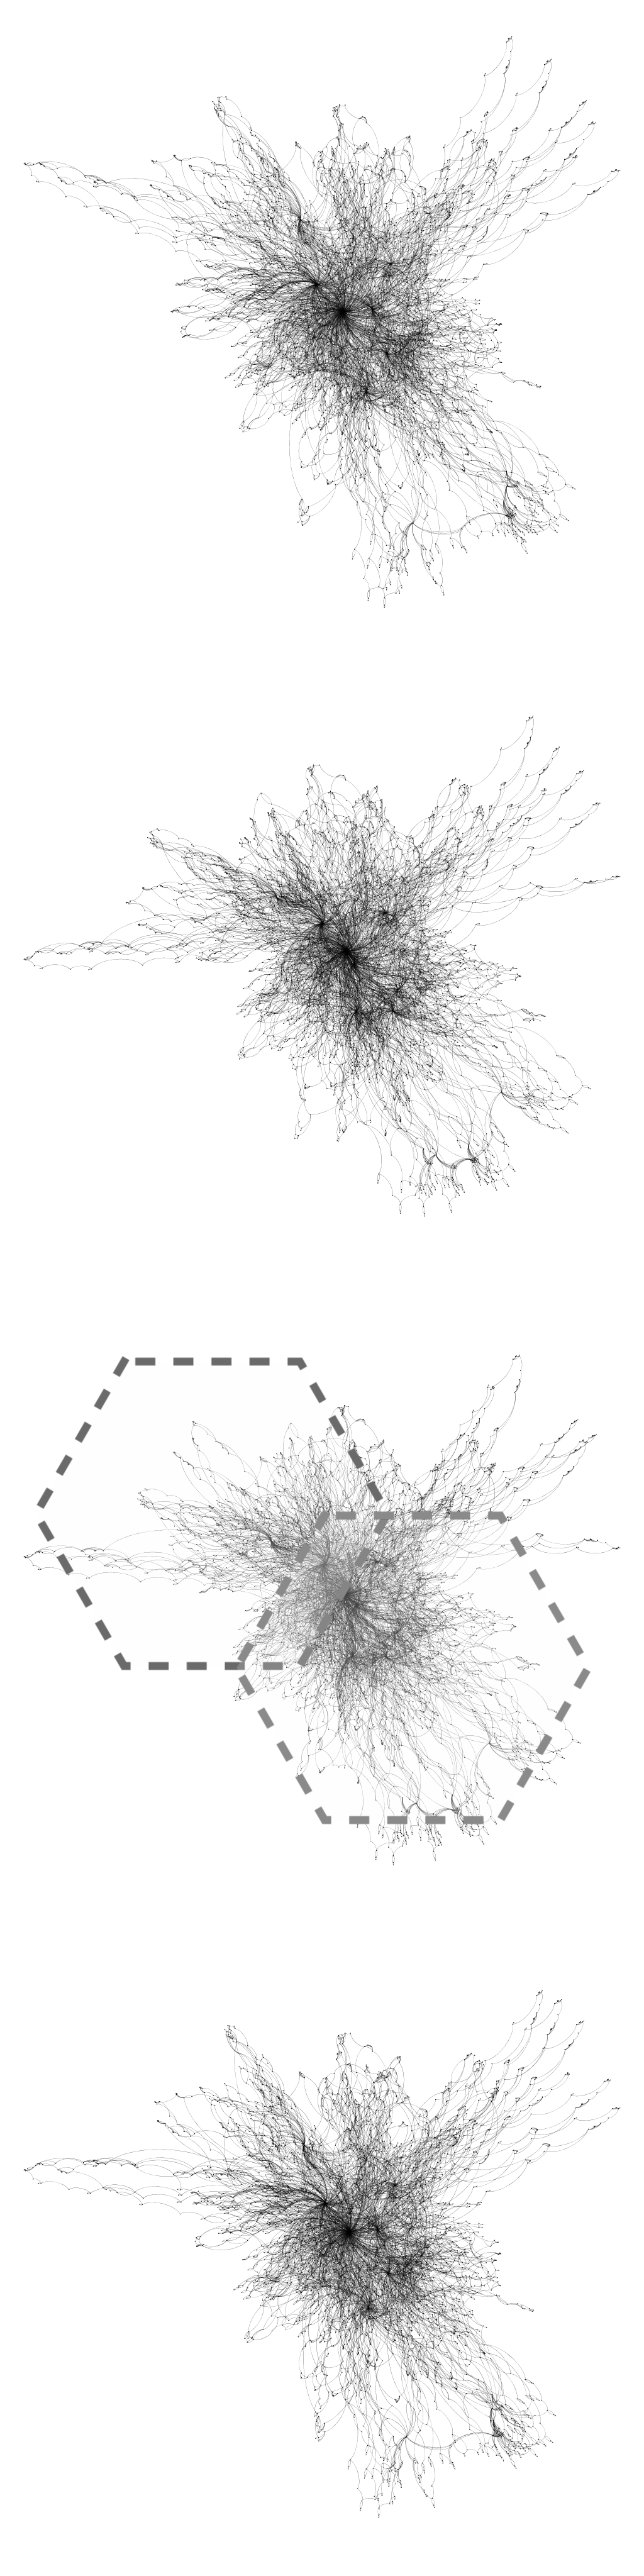
\includegraphics[width=\textwidth]{figures_c1/beijingtest/1.png}
     \caption{Group 1}
     \end{subfigure}
     \begin{subfigure}[b]{.2\textwidth}
         \centering
     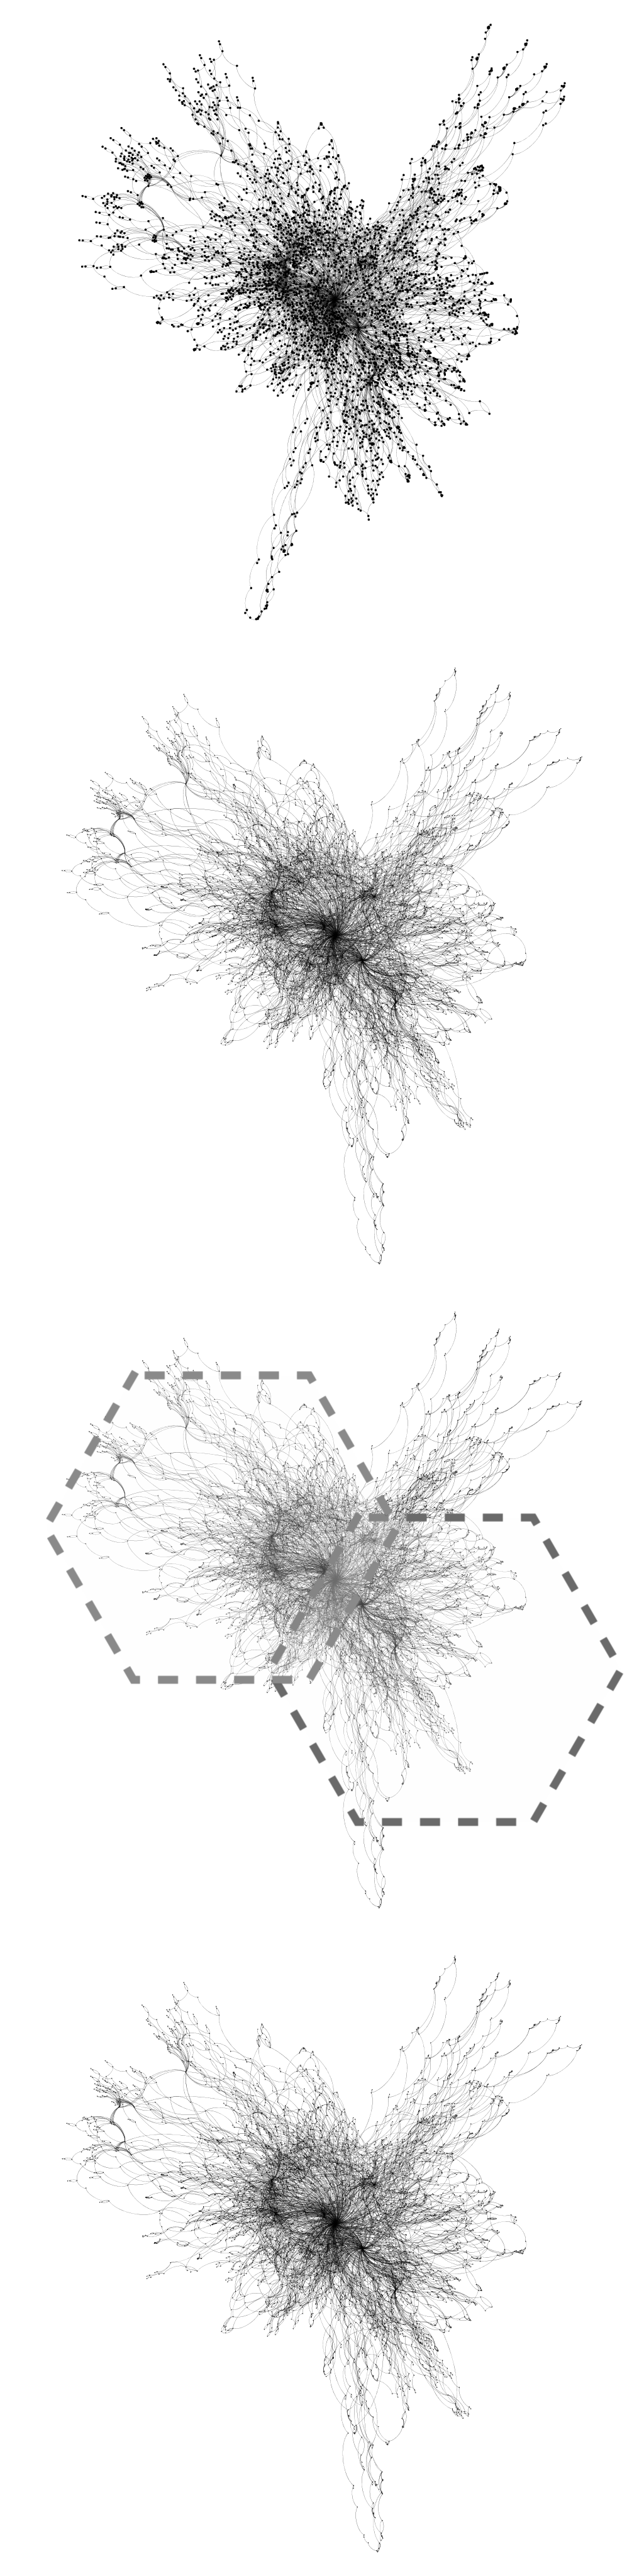
\includegraphics[width=\textwidth]{figures_c1/beijingtest/2.png}
     \caption{Group 2}
     \end{subfigure}
     \begin{subfigure}[b]{.2\textwidth}
         \centering
     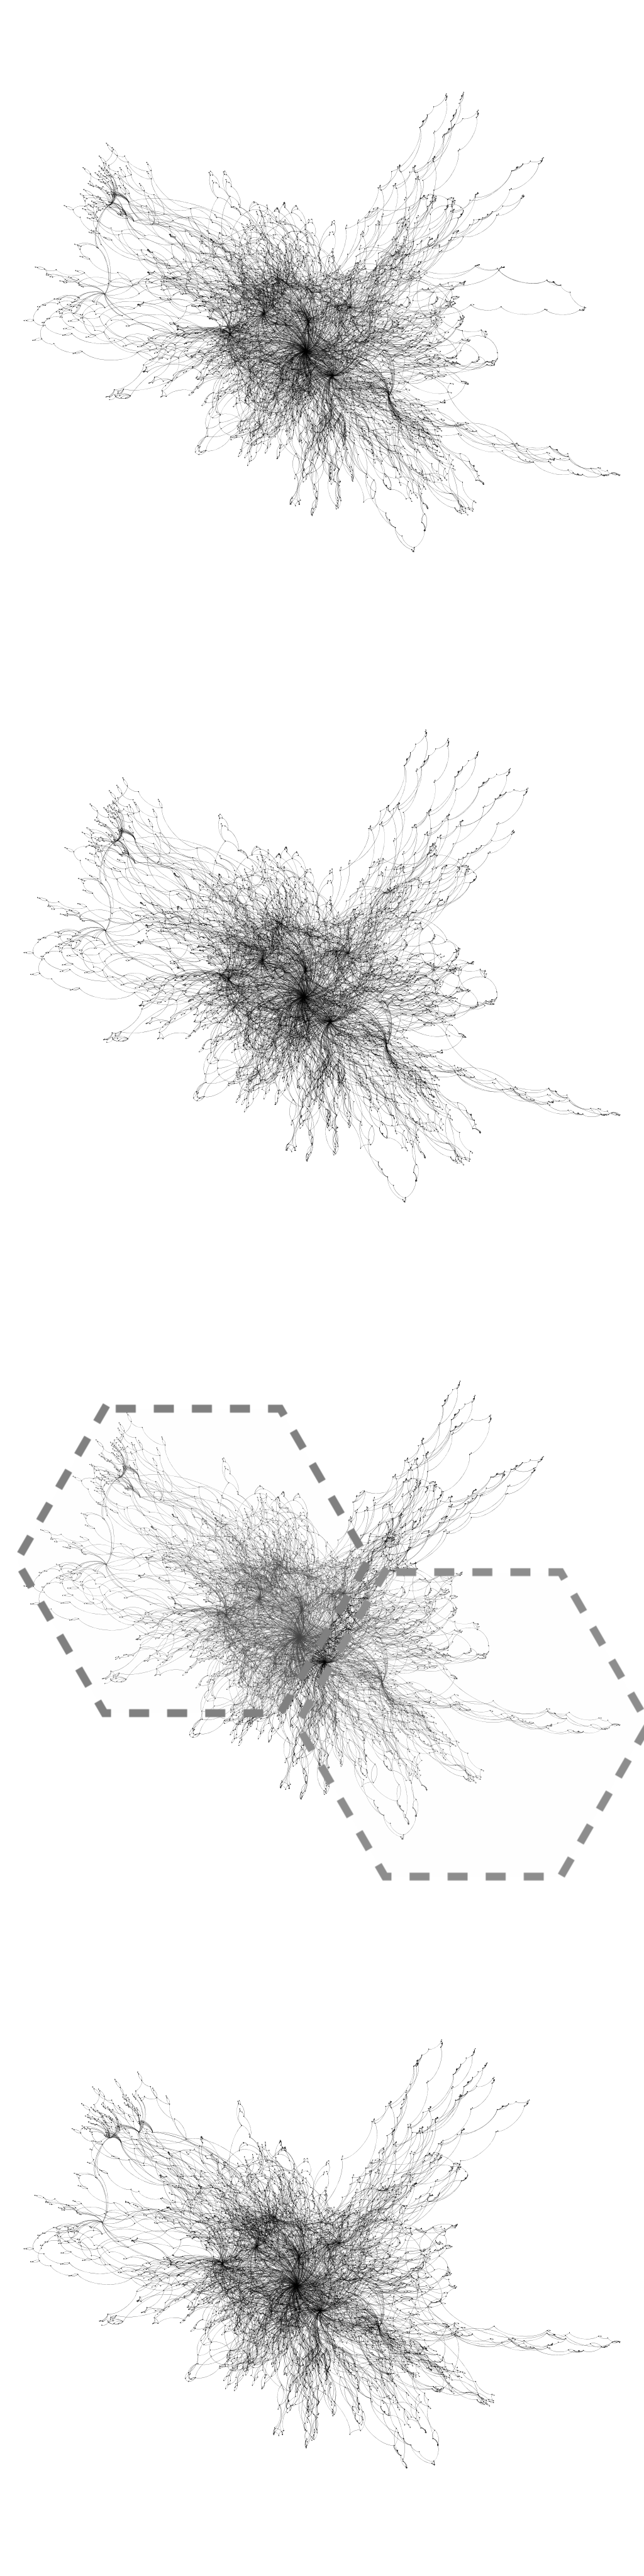
\includegraphics[width=\textwidth]{figures_c1/beijingtest/3.png}
     \caption{Group 3}
     \end{subfigure}
     \begin{subfigure}[b]{.2\textwidth}
         \centering
     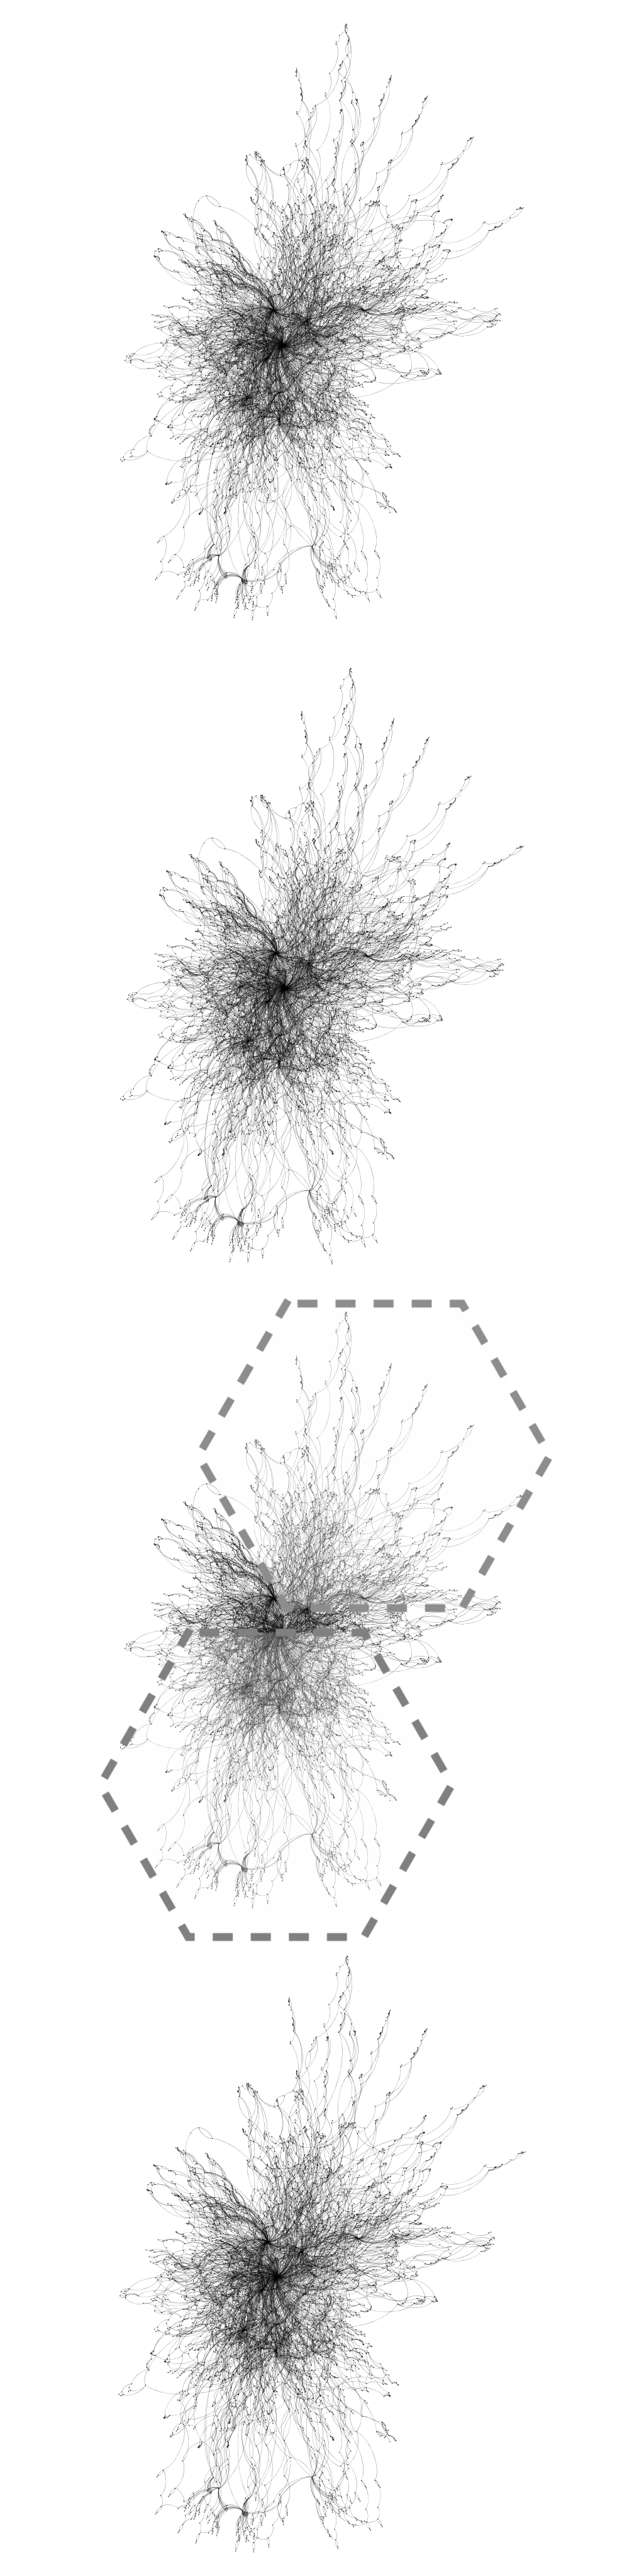
\includegraphics[width=\textwidth]{figures_c1/beijingtest/4.png}
     \caption{Group 4}
     \end{subfigure}
        \caption{\textbf{A selection of graphs corresponding to the labeled clusters in \autoref{fig:densty}}. These reveal that symmetric similarity between like-positioned points within the t-SNE output.  }
      \label{fig:densitypic}
\end{figure}

% \subsubsection{Location analysis and lifetime}
% In the previous subsection it was shown that the force atlas algorithm can be used to hi-light trends within the chemistry of a mechanism. Since the concentration change of a species depends on a range of factors which change throughout the length of a simulation, it follows that the force-directed graph generated for different timesteps may vary. Using the same setup as above we compare the network at noon (REF) and midnight (ref). 
% 
% \paragraph*{Diurnal Changes}\label{sec:diurnal}
% 
% 
% 
% 
% \paragraph*{Species Lifetime}
% 



\section{Summary}
Representing data in a visual format can be used to (utilise) the pattern recognition side of the human brain and alleviate the cognitive strain produced by numerical data. This is a technique used by the Samaritans (YEAR) with the use of cuneiform, and proved useful throughout. 

In designing a visualisation it is important to use storytelling and select metaphors familiar to the reader. This should be paired with the correct encoding, as to reduce the time spent trying to comprehend a figure, and increase the knowledge transfer. [ref chapter 1]

When considering relationships, one such analogy lies in the ball and stick analogy. Much like holding hands, this symbolises a similarity between connected items and is the basis of a mathematical graph, or network. Such representations can be applied to the chemical complexity seen in species within the atmosphere. 

In representing the chemistry within a mechanism as a graph we may visualise it with the use of a force-directed layout. These are in essence a simple physical simulation, whereupon each graph node is repelled (like-charge), and connected nodes joined by a spring-like attractive force. It is found that the force atlas 2 algorithm not only produces the best visual aesthetic, but also conceptual understanding. Using this it is possible to see patterns such as the the partitioning of each network into aromatic, terpene and straight chain chemistry. 

Although graph layouts have a range of local minima, the overall network structure of the MCM is constrained by its construction protocol (due to the allowed chemical reactions), and thus can be used to produce comparable graphs. This method of visualisation, in combination with interactive querying techniques, can aid in the comparison and understanding of large/complex chemistry simulations. This can be particularly useful in the explanation of specific interactions within a mechanism, or the exploration of temporal changes within a simulation. 

In the next chapter, I shall extend the graph metaphor for atmospheric chemistry systems beyond that of just visualisation. 
